\section{Penalised Linear Regression (Lasso, min/1se)} %4.3

In order to simplify the model by reducing the number of features whilst increasing the accuracy, Lasso Penalisation was applied. Using the \sys{glmnet} package, the weights of all features were presented as the change of Lambda value.

The ridge-trance figure (Figure \ref{4.2.2-NEW-PLR-ridge-trance-Log-Lambda}) shows that more and more coefficients become zero as the value of log lambda increases. In Lasso Penalisation, the features with poor performance are removed to reduce the complexity of the model.


\begin{figure}[htbp]
\center
  \begin{subfigure}{7.5cm}
    \centering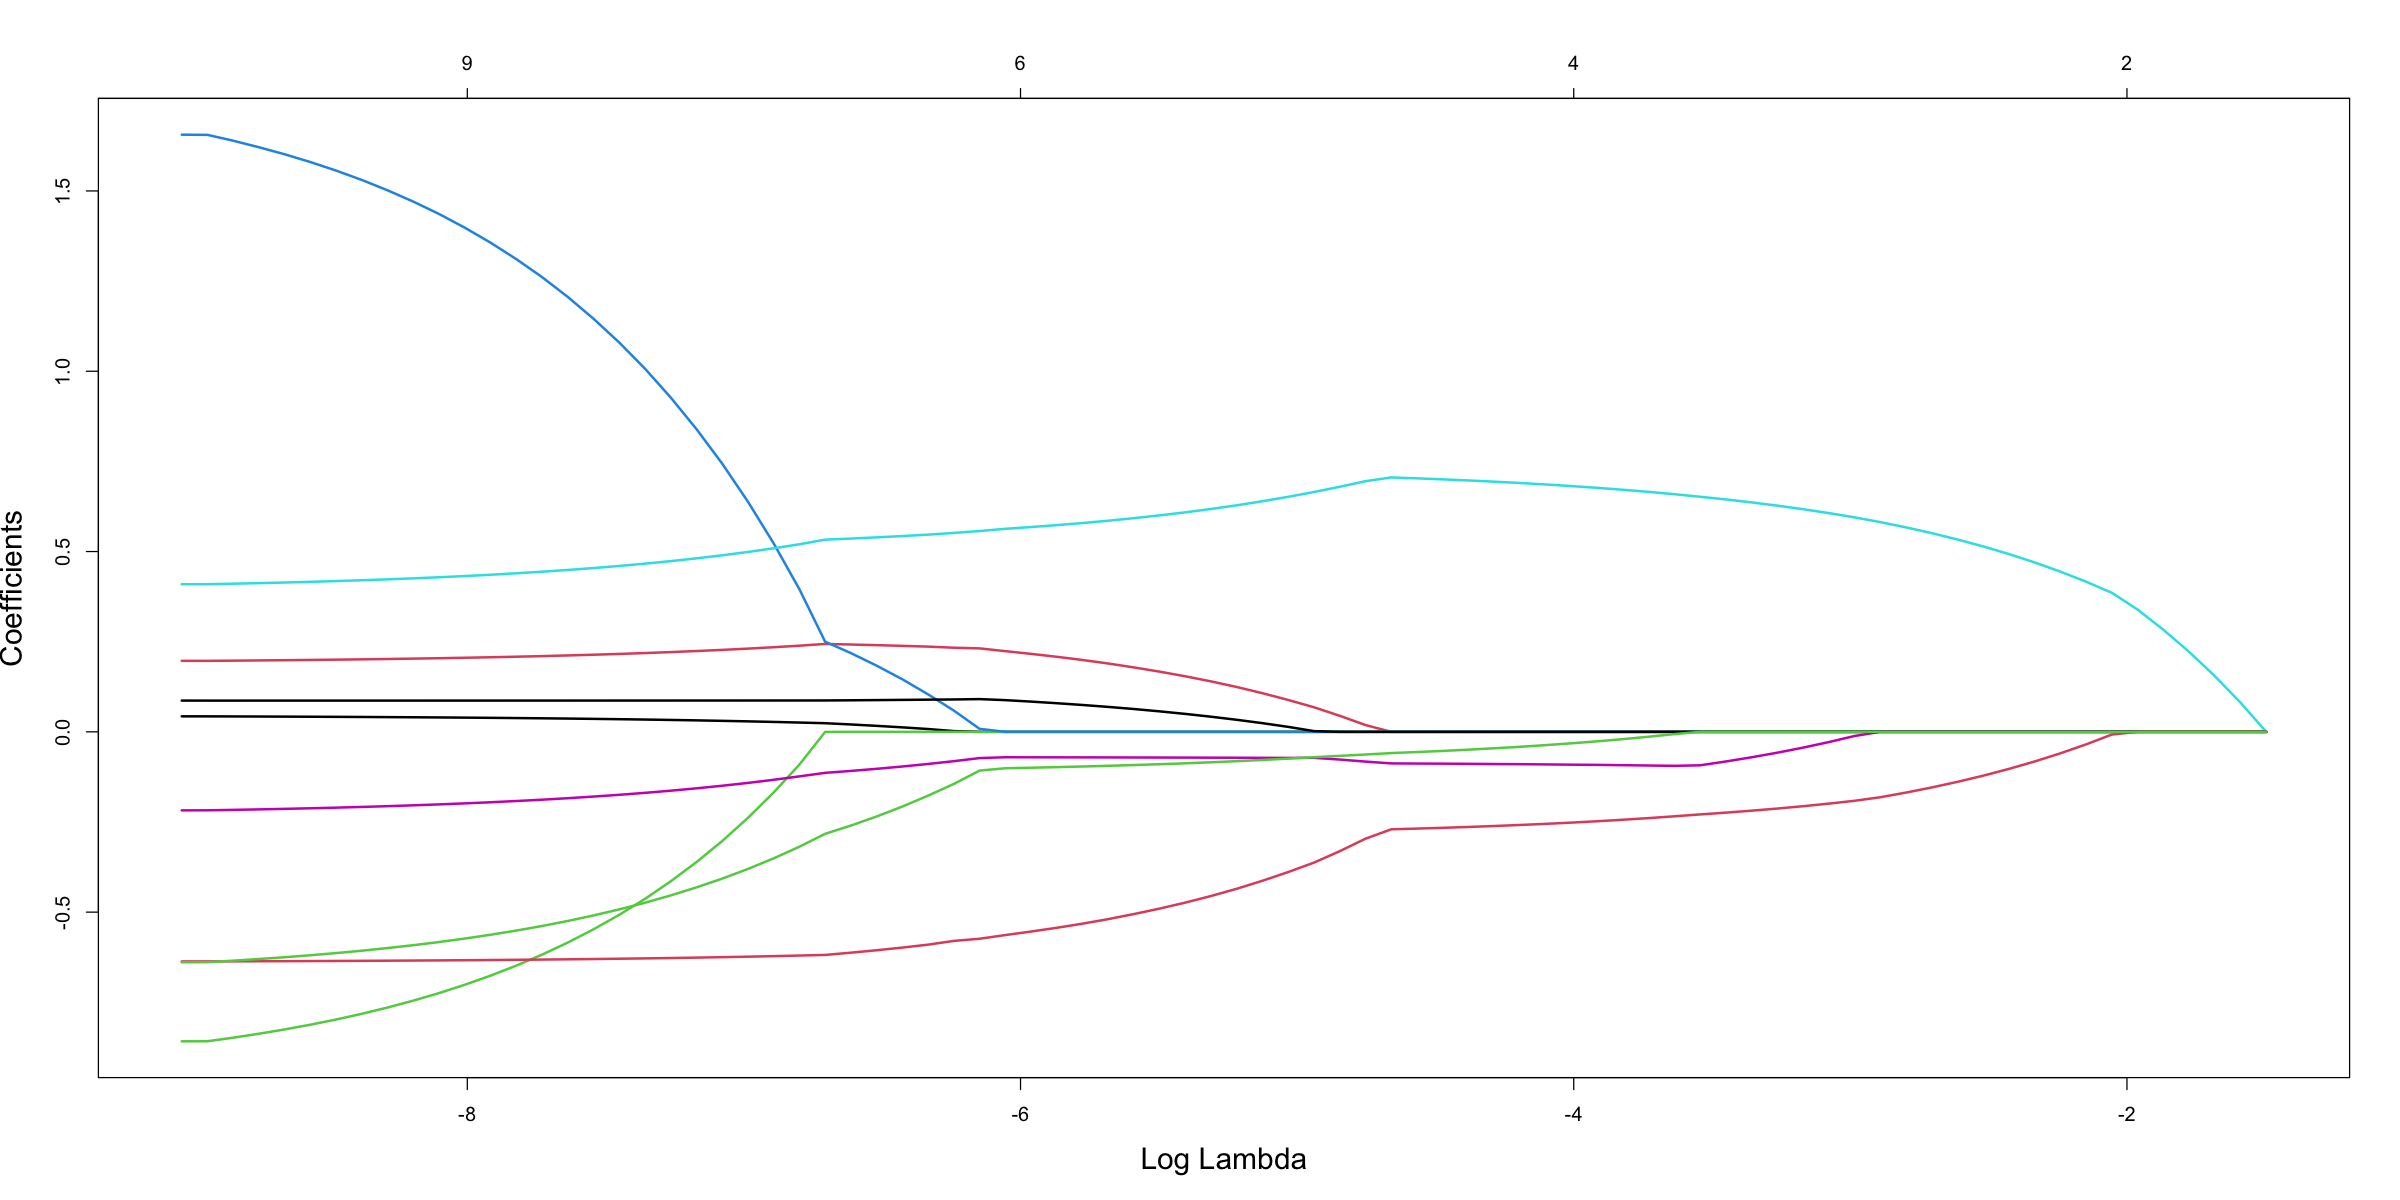
\includegraphics[width=7cm]{Figure/4.2.2-PLR-ridge-trance.png}
  \end{subfigure}
  \begin{subfigure}{7.5cm}
    \centering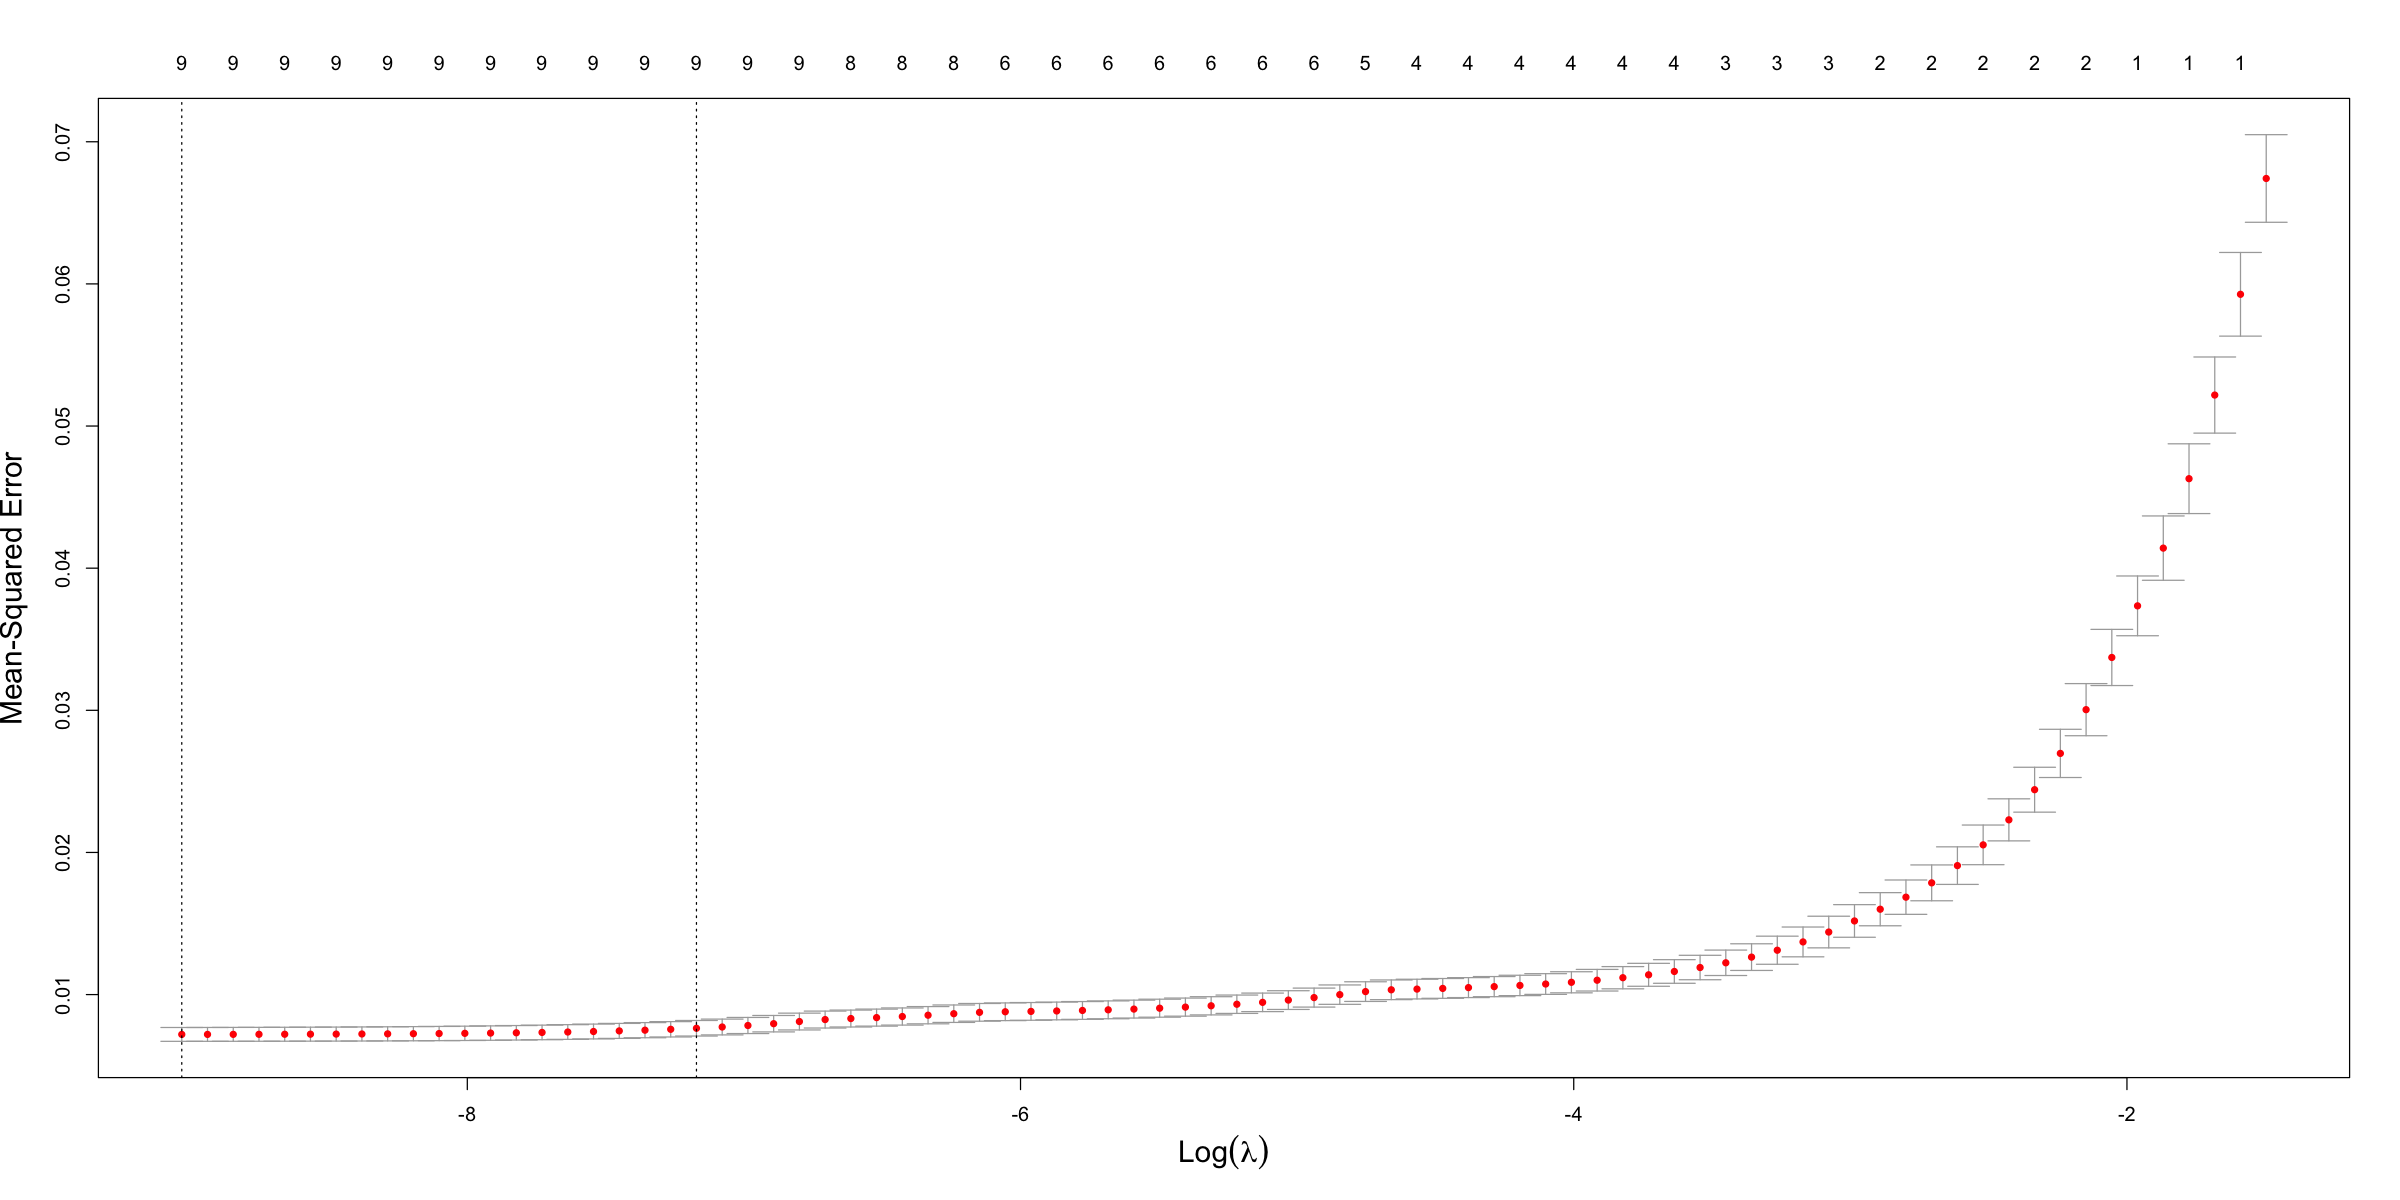
\includegraphics[width=7cm]{Figure/4.2.2-PLR-Log-Lambda-vs-Testing-Error.png}
  \end{subfigure}
  \caption{Left: Ridge trace diagram of Penalised Linear Regression. Right: Log Lambda vs Testing Error diagram of Penalised Linear Regression.}
  \label{4.2.2-NEW-PLR-ridge-trance-Log-Lambda}
\end{figure}


At this point, appropriate Lambda values were selected to output the weights of all features. In the selection, \sys{min} and \sys{1se} were applied respectively (Figure \ref{4.2.2-NEW-PLR-ridge-trance-Log-Lambda}).


Applying different options for the Lambda value, two different sets of results were obtained. When Lambda option was \sys{min}, the MSE value of the model was 0.00690, which was slightly less than the 0.00734 when Lambda option was \sys{1se}. 

The output result was demonstrated in Table \ref{4.2.2-PLR-para}. In this case, using \sys{1se} did not reduce the complexity of the model but the number of features. Therefore, \sys{min} was better than \sys{1se} in Lasso Penalisation in our project.

\begin{table}[htbp]
  \centering
  \footnotesize
  \begin{tabular}{p{5.75cm} | c | c}
  \toprule
  Coefficients: & min & 1se\\ %row 1
  \hline
    & 1 & 1\\
  (Intercept) & 0.71559335 & 0.66666336\\
  Rainfall & 0.04299020 & 0.03049067\\
  Daylight & 0.19686230 & 0.22725958\\
  Population & -0.85828586 & -0.30290499\\
  CO2 & 1.65605218 & 0.74378027\\
  Ozone & 0.40941811 & 0.48953790\\
  OceanTemperature\_NorthernHemisphere & -0.21778615 & -0.14950798\\
  LandTemperature\_NorthernHemisphere & 0.08669526 & 0.08684475\\
  MinTemperature\_NorthSlopeAlaska & -0.63667606 & -0.62486026\\
  GDP\_WORLD & -0.63894945 & -0.40706240\\
  \bottomrule
  \end{tabular}
  \caption{Hyper-parameters of Penalised Linear Regression.}
  \label{4.2.2-PLR-para}
\end{table}


In Linear Regression, the performance of test fitting was not ideal even it was optimised because of the lack of flexibility of the model. By adding a penalty term to the Linear Regression, the performance of test fitting was improved by both \sys{Min} and \sys{1SE} options. 


\begin{figure}[htbp]
\center
  \begin{subfigure}{7.5cm}
    \centering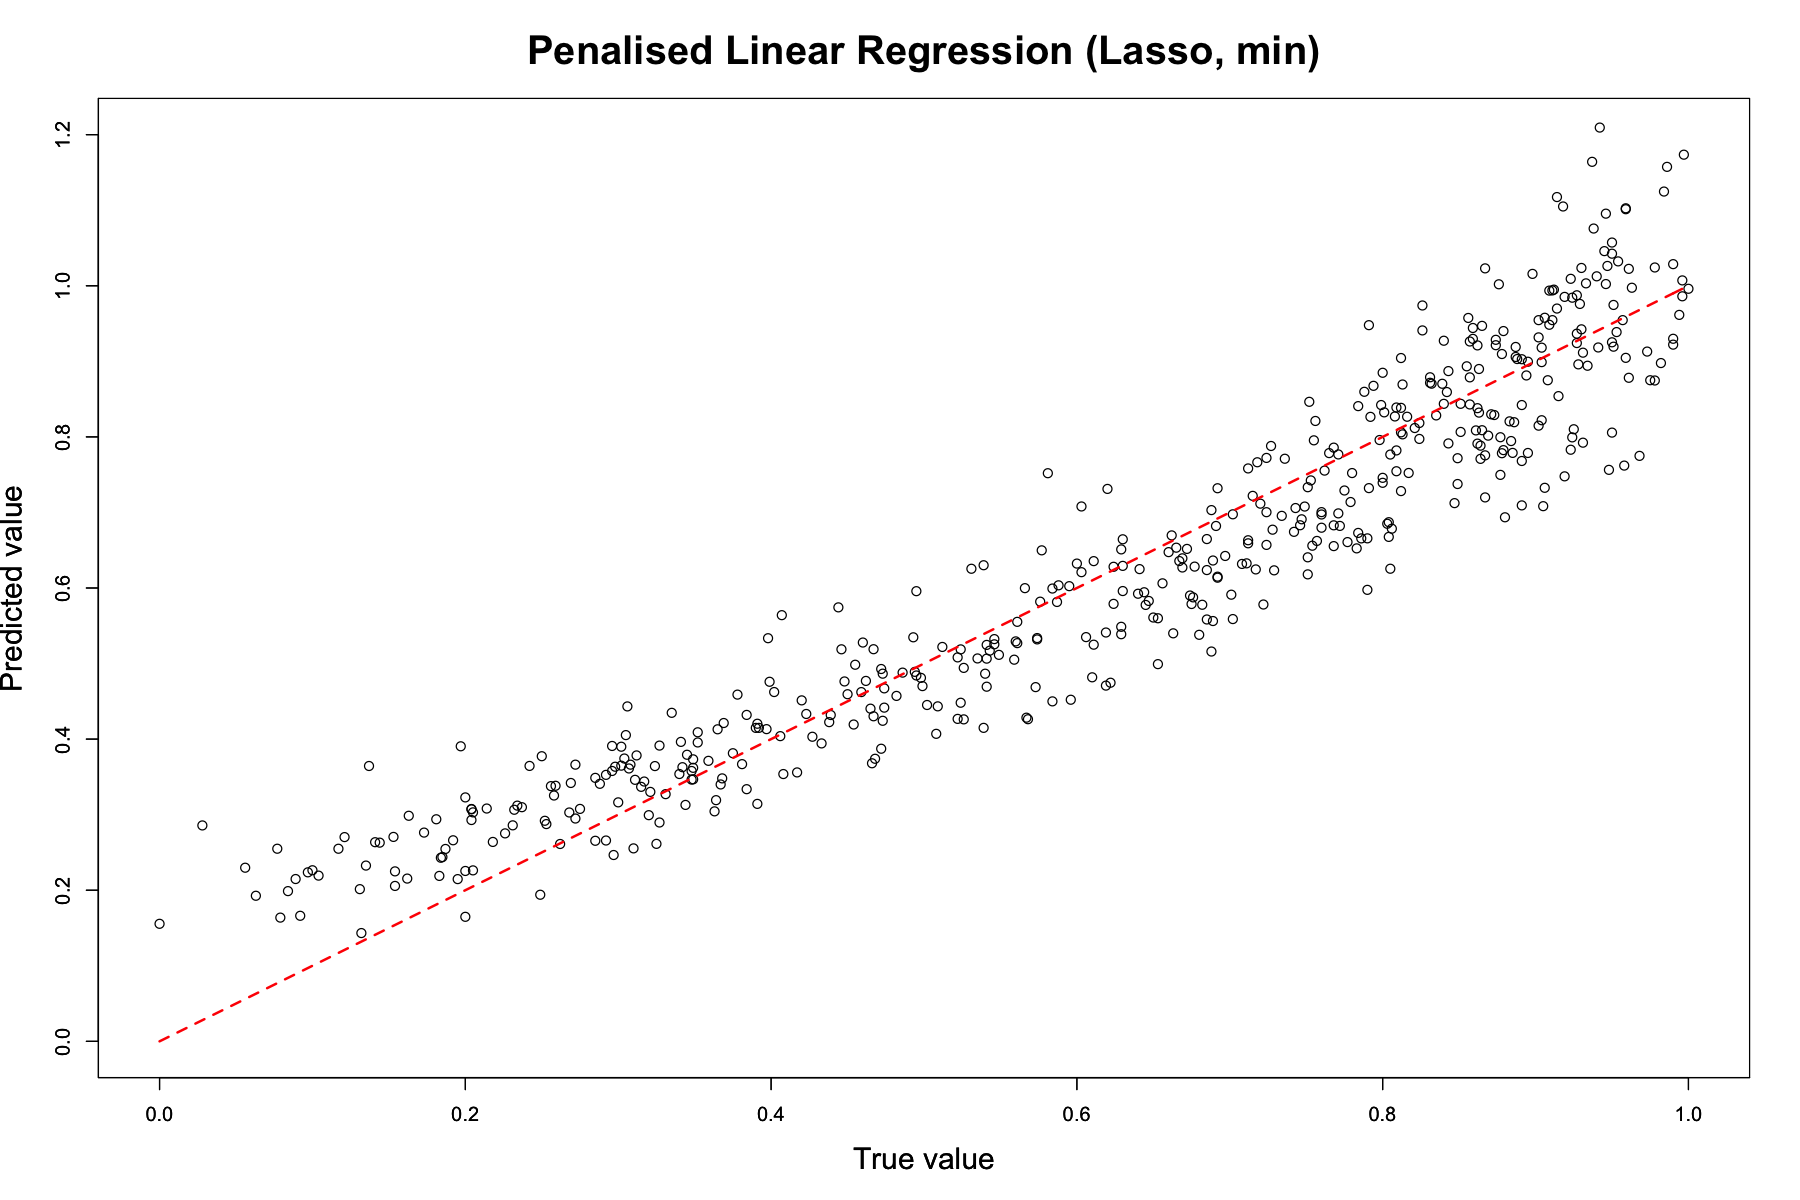
\includegraphics[width=7cm]{Figure/4.2.2-PLR-min.png}
  \end{subfigure}
  \begin{subfigure}{7.5cm}
    \centering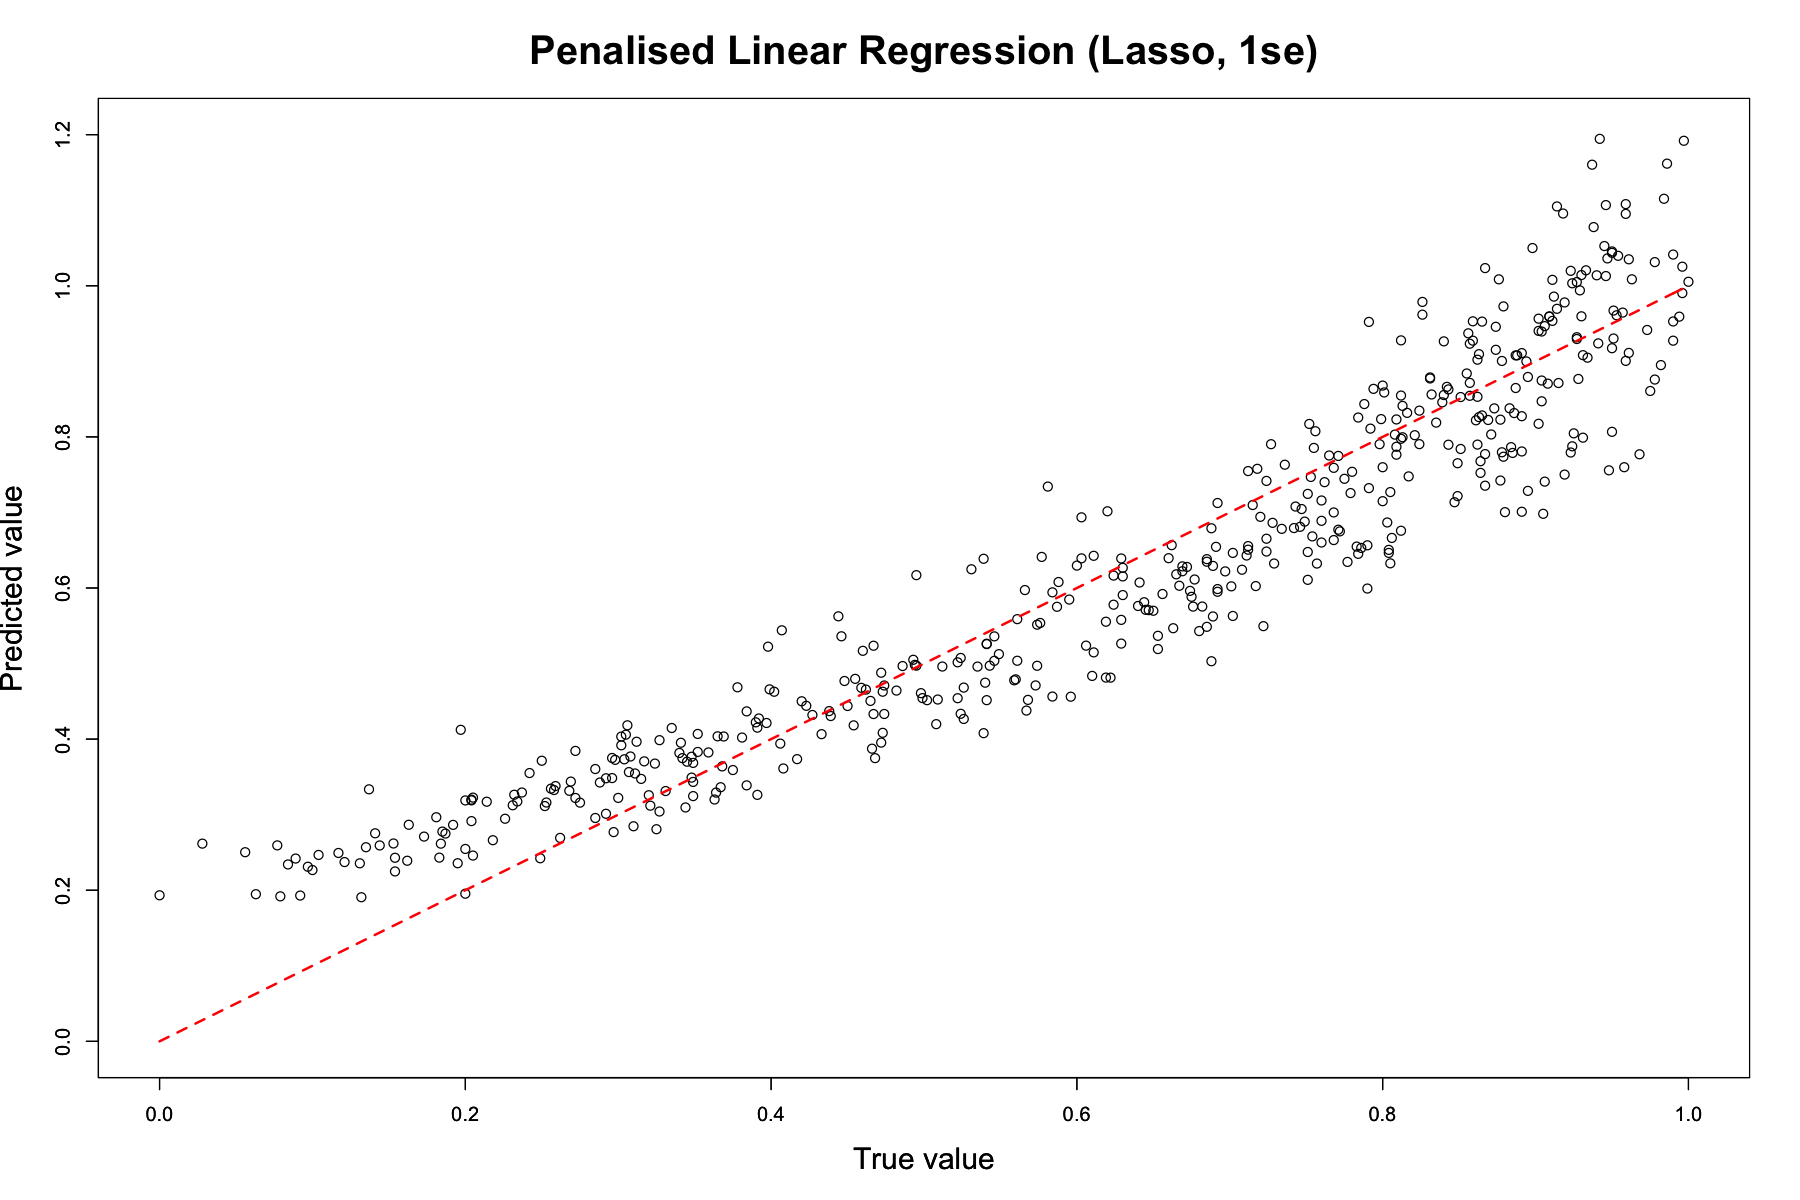
\includegraphics[width=7cm]{Figure/4.2.2-PLR-1se.png}
  \end{subfigure}
  \caption{\textbf{Left}: The predicted Arctic sea ice extent value vs the real Arctic sea ice extent value with \textbf{Penalised Linear Regression} (Lasso, \textbf{min}). The red referenced dotted line represents the straight line y=x. Mean Square Error (MSE) is \textbf{0.00690}. \textbf{Right}: The predicted Arctic sea ice extent value vs the real Arctic sea ice extent value with \textbf{Penalised Linear Regression} (Lasso, \textbf{1se}). The red referenced dotted line represents the straight line y=x. Mean Square Error (MSE) is \textbf{0.00732}.}
  \label{4.2.2-PLR-min-1se}
\end{figure}

\newpage